\documentclass[fleqn]{jbook}
\usepackage{physpub}

\begin{document}

\begin{question}{専攻 問題1}{}

井戸型ポテンシャルの中に置かれた電子系の運動を考える。電子の運動は$x$
軸方向のみ考えればよく、それに直行する方向の運動は考えない。
ポテンシャルは$-a<x<a$($a$は正の定数)で$0$で、$x=-a$および$x=+a$に無限に高
い壁をもつ。$i$番目($i=1,2,..$)の電子の座標を$x_i$とし、そのスピンを
$\vec{s_i}$と表わす。またその電子のスピン波動関数については、上向きを
$u_\uparrow(i)$、下向きを$u_\downarrow(i)$とする。電子の質量を$m$とし
て、以下の設問に答えよ。

\begin{subquestions}
\SubQuestion
  1個の電子をこの井戸型ポテンシャルの中に入れた時のエネルギー固有値を
  求めよ。ただし、下から$n$番目($n=1,2,..$)のものを$E_n$とせよ。

\SubQuestion
  電子はフェルミ粒子である。この事実は、この井戸型ポテンシャル内に2個
  の電子を入れた時に、それらの波動関数にどのような条件を課すか、述べよ。

\SubQuestion
  2個の電子をこの井戸型ポテンシャル内に入れたところ、最も低いエネルギ
  ー固有状態が実現された。この時のエネルギー固有値を求め、その状態での
  電子系の波動関数を、スピン部分まで含めて示せ。さらに、電子の合成スピ
  ン演算子
  \[
    \vec{S}=\vec{s_1}+\vec{s_2}
  \] 
  に対して、この状態での$(\vec{S} \cdot \vec{S})$の期待値を求めよ。
  以後$(\cdot)$は内積を表わす。

\SubQuestion
  設問3と同じ場合で、2番目に低いエネルギー固有状態が実現されていたと
  する。このエネルギー固有値に属する系の固有状態には、どのようなものが
  あり得るか。スピン部分まで含め、それらの波動関数を示せ。

\SubQuestion
  ここで電子間に
  \[
    V = f \times (\vec{s_1} \cdot \vec{s_2}) \times \delta(x_{1}-x_{2})
  \]
  という相互作用が働くとする。ただし$f$は結合定数で、十分に小さい正の
  値をとるものとし、$\delta()$はデルタ関数を表わす。この相互作用が加
  わったとき、設問3で求めた状態のエネルギー固有値の変化を計算せよ。

\SubQuestion
  設問5の相互作用$V$が働いたとき、設問3の状態と、設問4で考えた状態
  (複数でもよい)は、どのように混ざるか答えよ。

\end{subquestions}

\end{question}
\begin{answer}{専攻 問題1}{}

\begin{subanswers}
\SubAnswer

Schr\"odinger方程式
\[
-\frac{\hbar^{2}}{2m}\frac{d^{2}}{dx^{2}}\psi(x) = E\psi(x) \qquad (|x|<a)
\]
\[
\psi(a)=\psi(-a)=0
\]
を解けばいい。解は、n=1,2,...として、
\[
\psi_{n}(x)=
\left\{
	\begin{array}{rl}
	\frac{1}{\sqrt{a}}\cos(\frac{n{\pi}x}{2a}) & n:奇数 \\
	\frac{1}{\sqrt{a}}\sin(\frac{n{\pi}x}{2a}) & n:偶数
	\end{array}
\right.
\]
\[
E_{n}=\frac{\hbar^{2}\pi^{2}n^{2}}{8ma^{2}}
\]
となる。

\SubAnswer

「電子の入れ換えに対し、波動関数が反対称である」という条件。


\SubAnswer

 \parbox[t]{100mm}{
 右図のように下から2つの電子をつめればエネルギー固有値最小。
 \[
 E_{total}=E_{1}+E_{1}=\frac{\hbar^{2}\pi^{2}}{4ma^{2}}
 \]
 }
 \parbox[t]{50mm}{
 \begin{center}
  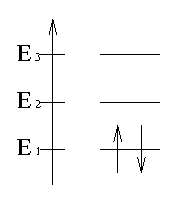
\includegraphics[clip,height=30mm,width=30mm]{1998phy1-1.eps}
 \end{center}
 }

 
さて、波動関数は軌道の波動関数とスピンの波動関数との積であり、$\psi_{total}(1,2)=\psi_{orbit}\psi_{spin}$のようにかく。
今は、
\[
\psi_{orbit}=\psi_{1}(x_{1})\psi_{1}(x_{2})=\frac{1}{a}\cos\left(\frac{{\pi}x_{1}}{2a}\right)\cos\left(\frac{{\pi}x_{2}}{2a}\right)
\]
で、電子の入れ換えに対し対称である。すると設問2の条件から$\psi_{spin}$は反対称でなくてはならない。よって、
\[
\psi_{spin}=\frac{1}{\sqrt{2}}[u_{\uparrow}(1)u_{\downarrow}(2)-u_{\downarrow}(1)u_{\uparrow}(2)]
\]
とわかる。

まとめると、
\[
\psi_{total}(1,2)=\frac{1}{a}\cos\left(\frac{{\pi}x_{1}}{2a}\right)\cos\left(\frac{{\pi}x_{2}}{2a}\right)\frac{1}{\sqrt{2}}[u_{\uparrow}(1)u_{\downarrow}(2)-u_{\downarrow}(1)u_{\uparrow}(2)]
\]

さて、合成スピン(大きさ$S$、z成分$S_{z}$)の波動関数は、

\begin{table}[h]
\[
	\begin{array}{lcc}
	 & S=1(対称) & S=0(反対称) \\
	S_{z}=1 & u_{\uparrow}(1)u_{\uparrow}(2) & \\
	S_{z}=0 & \frac{u_{\uparrow}(1)u_{\downarrow}(2)+u_{\downarrow}(1)u_{\uparrow}(2)}{\sqrt{2}} &\frac{u_{\uparrow}(1)u_{\downarrow}(2)-u_{\downarrow}(1)u_{\uparrow}(2)}{\sqrt{2}} \\
	S_{z}=-1 & u_{\downarrow}(1)u_{\downarrow}(2) &
	\end{array}
\]
\caption{合成スピンの波動関数}
\end{table}

なので、今の$\psi_{spin}$は$S=0$,$S_{z}=0$の固有関数。
\[
S^{2}\psi_{total}(1,2)=0(0+1)\psi_{total}(1,2)=0
\]
より、
\[
<S^{2}>=0
\]

\SubAnswer


\parbox[t]{90mm}{
たとえば右図のように$E_{1}$の所に電子1つ、$E_{2}$の所に電子1つのときである。$\psi_{total}$が反対称になるために、$\psi_{orbit}$が対称で$\psi_{spin}$が反対称となるか、$\psi_{orbit}$が反対称で$\psi_{spin}$が対称とならなければならない。$\psi_{spin}$の対称性の可能性は表1のようであるので、あり得る$\psi_{total}$は次の4つとなる。}
\parbox[t]{60mm}{
\begin{center}
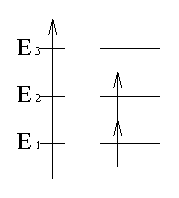
\includegraphics[clip,height=30mm,width=30mm]{1998phy1-2.eps}
\end{center}
}


\begin{eqnarray*}
\psi(2a,1,1) &\equiv& \frac{1}{\sqrt{2}}[\psi_{1}(x_{1})\psi_{2}(x_{2})-\psi_{2}(x_{1})\psi_{1}(x_{2})]u_{\uparrow}(1)u_{\uparrow}(2) \\
\psi(2a,1,0) &\equiv& \frac{1}{\sqrt{2}}[\psi_{1}(x_{1})\psi_{2}(x_{2})-\psi_{2}(x_{1})\psi_{1}(x_{2})]\frac{1}{\sqrt{2}}[u_{\uparrow}(1)u_{\downarrow}(2)+u_{\downarrow}(1)u_{\uparrow}(2)] \\
\psi(2a,1,-1) &\equiv& \frac{1}{\sqrt{2}}[\psi_{1}(x_{1})\psi_{2}(x_{2})-\psi_{2}(x_{1})\psi_{1}(x_{2})]u_{\downarrow}(1)u_{\downarrow}(2) \\
\psi(2s,0,0) &\equiv& \frac{1}{\sqrt{2}}[\psi_{1}(x_{1})\psi_{2}(x_{2})+\psi_{2}(x_{1})\psi_{1}(x_{2})]\frac{1}{\sqrt{2}}[u_{\uparrow}(1)u_{\downarrow}(2)-u_{\downarrow}(1)u_{\uparrow}(2)]
\end{eqnarray*}

ここで、$\psi(*\#,*,*)$の第一引数は系のエネルギーが下から$*$番目で軌道部分の対称性が\#(aは反対称、sは対称)をあらわし、第二引数は$S=*$,第三引数は$S_{z}=*$をあらわす。

\SubAnswer

設問3でもとめた$\psi_{total}(1,2)$は設問4の記法で$\psi(1s,0,0)$とかける。
\[
S_{1}^{2}\psi(1s,0,0)=S_{2}^{2}\psi(1s,0,0)=\frac{3}{4}\psi(1s,0,0)
\]
\[
S^{2}\psi(1s,0,0)=0
\]
であるので、
\begin{equation}
\mathbf{S_{1}{\cdot}S_{2}}\psi(1s,0,0)=-\frac{3}{4}\psi(1s,0,0)
\end{equation}
ここで$S^{2}=\mathbf{(S_{1}+S_{2})\cdot(S_{1}+S_{2})}=S_{1}^{2}+S_{2}^{2}+2\mathbf{S_{1}{\cdot}S_{2}}$より、
\[
\mathbf{S_{1}{\cdot}S_{2}}=\frac{S^{2}-S_{1}^{2}-S_{2}^{2}}{2}
\]
となることをもちいた。

$V=f\mathbf{S_{1}{\cdot}S_{2}}\delta(x_{1}-x_{2})$という摂動がかかったときの$\psi(1s,0,0)$のエネルギー固有値の1次の変化${\Delta}E_{total}$は
\begin{eqnarray*}
{\Delta}E_{total} &=& \langle 1s,0,0|V|1s,0,0 \rangle \\
		&\stackrel{(1)}{=}& -\frac{3}{4}f\langle 1s,0,0|\delta(x_{1}-x_{2})|1s,0,0 \rangle \\
		&=& -\frac{3}{4}f \int dx_{1}dx_{2}\psi_{1}(x_{1})^{2}\psi_{1}(x_{2})^{2}\delta(x_{1}-x_{2}) \\
		&=& -\frac{3}{4}f \int_{-a}^{a} dx \psi_{1}(x)^{4} \\
		&=& -\frac{3}{4}f \frac{1}{a^{2}} \int_{-a}^{a} dx \cos^{4}\left(\frac{{\pi}x}{2a}\right) \\
		&=& -\frac{9f}{16a}
\end{eqnarray*}


\SubAnswer

\begin{picture}(300,100)
\put(65,0){\vector(0,1){100}}

\put(0,67){$\varepsilon_{2}=E_{1}+E_{2}$}
\put(60,70){\line(1,0){10}}
\put(80,70){\line(1,0){50}}
	\put(90,60){$|2a,1,1 \rangle$}
\put(150,70){\line(1,0){50}}
	\put(160,60){$|2a,1,0 \rangle$}
\put(220,70){\line(1,0){50}}
	\put(225,60){$|2a,1,-1 \rangle$}
\put(290,70){\line(1,0){50}}
	\put(300,60){$|2s,0,0 \rangle$}

\put(20,27){$\varepsilon_{1}=2E_{1}$}
\put(60,30){\line(1,0){10}}
\put(150,30){\line(1,0){50}}
	\put(160,20){$|1s,0,0 \rangle$}
\end{picture}

以上5つの状態ベクトルがどのように混ざるか考える。

\begin{eqnarray*}
\langle 2a,*,*|V|*,*,* \rangle &=& 
\underbrace{
\langle *,*|f\mathbf{S_{1}\cdot S_{2}}|*,* \rangle
}_{スピン部分} \\
& &\qquad\int dx_{1}dx_{2}\frac{1}{\sqrt{2}}
\underbrace{
[\psi_{1}(x_{1})\psi_{2}(x_{2})-\psi_{2}(x_{1})\psi_{1}(x_{2})]
}_{x_{1}=x_{2}で0} \\
& & \qquad \qquad \delta(x_{1}-x_{2})
\underbrace{
g(x_1,x_2)
}_{適当な関数} \\
&=&0
\end{eqnarray*}
\begin{eqnarray*}
\langle 2s,0,0|V|1s,0,0 \rangle &=&
\langle 0,0|f\mathbf{S_{1}\cdot S_{2}}|0,0 \rangle \\
& &\qquad \int dx_{1}dx_{2}\frac{1}{\sqrt{2}}[\psi_{1}(x_{1})\psi_{2}(x_{2})+\psi_{2}(x_{1})\psi_{1}(x_{2})] \\
& &\qquad \qquad \psi_{1}(x_{1})\psi_{1}(x_{2})\delta(x_{1}-x_{2}) \\
&=&\sqrt{2}\langle 0,0|f\mathbf{S_{1}\cdot S_{2}}|0,0 \rangle \int_{-a}^{a}\psi_{1}(x)^{3}\psi_{2}(x)dx \\
&=&\frac{\sqrt{2}f}{a^{2}}\langle 0,0|\mathbf{S_{1}\cdot S_{2}}|0,0 \rangle \int_{-a}^{a} 
\underbrace{
\cos^{3}\left(\frac{{\pi}x}{2a}\right)\sin\left(\frac{{\pi}x}{a}\right)dx
}_{奇関数} \\
&=&0
\end{eqnarray*}

より、以上5つの状態ベクトルから異なる2つを選んだ時、その行列要素($V$をはさんだもの)が0となるので、以上の5つの状態は$V$によって混ざらない。

\end{subanswers}
\end{answer}

\end{document}
